\documentclass[runningheads]{llncs}

% ---------------------------------------------------------------
% Include basic ECCV package
 
% TODO REVIEW: Insert your submission number below by replacing '*****'
% TODO FINAL: Comment out the following line for the camera-ready version
\usepackage[review,year=2026,ID=*****]{eccv}
% TODO FINAL: Un-comment the following line for the camera-ready version
%\usepackage{eccv}

% OPTIONAL: Un-comment the following line for a version which is easier to read
% on small portrait-orientation screens (e.g., mobile phones, or beside other windows)
%\usepackage[mobile]{eccv}


% ---------------------------------------------------------------
% Other packages

% Commonly used abbreviations (\eg, \ie, \etc, \cf, \etal, etc.)
\usepackage{eccvabbrv}

% Include other packages here, before hyperref.
\usepackage{graphicx}
\usepackage{booktabs}
\usepackage{algorithm}


\usepackage{algpseudocode}
% The "axessiblity" package can be found at: https://ctan.org/pkg/axessibility?lang=en
\usepackage[accsupp]{axessibility}  % Improves PDF readability for those with disabilities.

\usepackage{multirow}
% ---------------------------------------------------------------
% Hyperref package

% It is strongly recommended to use hyperref, especially for the review version.
% Please disable hyperref *only* if you encounter grave issues.
% hyperref with option pagebackref eases the reviewers' job, but should be disabled for the final version.
%
% If you comment hyperref and then uncomment it, you should delete
% main.aux before re-running LaTeX.
% (Or just hit 'q' on the first LaTeX run, let it finish, and you
%  should be clear).

% TODO FINAL: Comment out the following line for the camera-ready version
%\usepackage[pagebackref,breaklinks,colorlinks,citecolor=eccvblue]{hyperref}
% TODO FINAL: Un-comment the following line for the camera-ready version
\usepackage{hyperref}

% Support for ORCID icon
\usepackage{orcidlink}


\begin{document}

% ---------------------------------------------------------------
% TODO REVIEW: Replace with your title
\title{Agentic Causal Disentanglement Framework: \\ Reversing the Generalization–Tail Trade-Off via Clinical Knowledge Integration in Medical AI} 

% TODO REVIEW: If the paper title is too long for the running head, you can set
% an abbreviated paper title here. If not, comment out.
\titlerunning{Abbreviated paper title}

% TODO FINAL: Replace with your author list. 
% Include the authors' OCRID for the camera-ready version, if at all possible.
\author{First Author\inst{1}\orcidlink{0000-1111-2222-3333} \and
Second Author\inst{2,3}\orcidlink{1111-2222-3333-4444} \and
Third Author\inst{3}\orcidlink{2222--3333-4444-5555}}

% TODO FINAL: Replace with an abbreviated list of authors.
\authorrunning{F.~Author et al.}
% First names are abbreviated in the running head.
% If there are more than two authors, 'et al.' is used.

% TODO FINAL: Replace with your institution list.
\institute{Princeton University, Princeton NJ 08544, USA \and
Springer Heidelberg, Tiergartenstr.~17, 69121 Heidelberg, Germany
\email{lncs@springer.com}\\
\url{http://www.springer.com/gp/computer-science/lncs} \and
ABC Institute, Rupert-Karls-University Heidelberg, Heidelberg, Germany\\
\email{\{abc,lncs\}@uni-heidelberg.de}}

\maketitle


\begin{abstract}
Deep learning models deployed in clinical settings face two main challenges: \textbf{Domain Generalization (DG)} and \textbf{Long-Tailed Visual Recognition (LT-VR)}. DG mandates learning domain-invariant features to perform robustly across heterogeneous acquisition protocols and patient populations. We formally investigate the theoretical trade-off where gradient alignment objectives prioritized by DG methods undermine the class-aware optimization necessary for LT-VR . To resolve this issue, we introduce the \textbf{Agentic Causal Disentanglement (ACD) Framework}, a novel modular architecture that integrates explicit \textbf{clinical knowledge/expertise} sourced autonomously from sonographers, radiologists, and specialists as a causal intervention tool. ACD orchestrates three specialized agents: the \textbf{Clinical Reasoning Agent (CRA)}, the \textbf{Causal Disentanglement Agent (CDA)}, and the \textbf{Code Generation Agent (CGA)}. This integration of domain-specific, causal knowledge effectively \textbf{decouples the DG and LT objectives}. Evaluated across \textbf{10 diverse medical imaging datasets} spanning \textbf{4 modalities}, the ACD Framework overall achieves an average \textbf{10.3\% performance improvement} across multi-domain and in-domain long-tailed tasks. 
\end{abstract}

\section{Introduction}
%\begin{figure}[t]
%    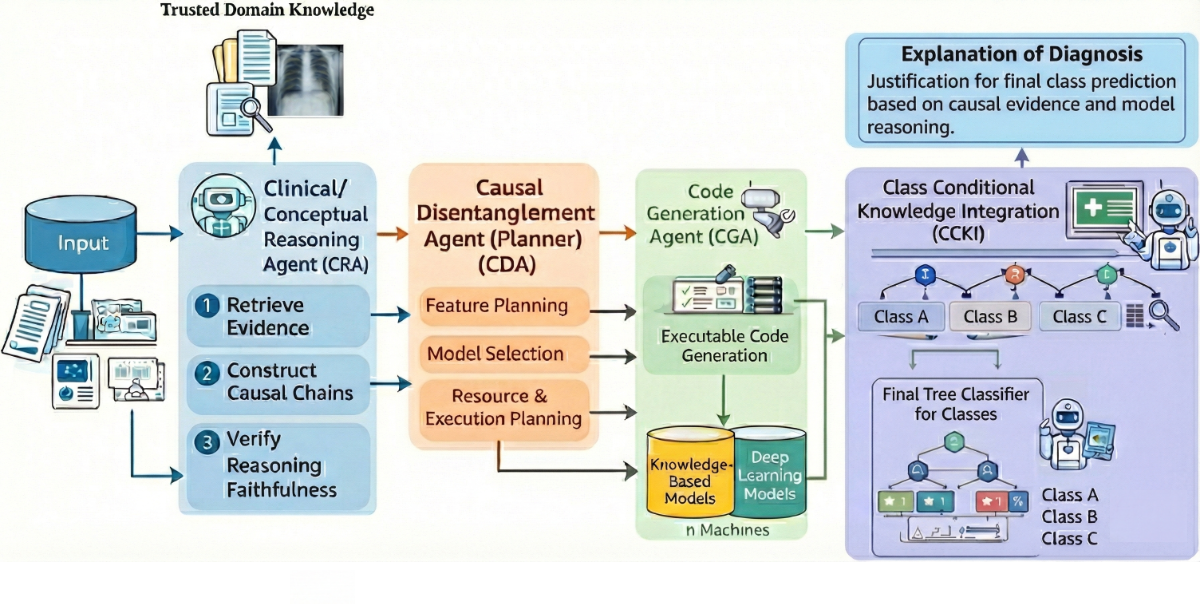
\includegraphics[width=0.5\textwidth]{main2.png}
%\caption{Overview of the proposed \textbf{ACD} agentic framework for knowledge  integrated classification.}

    \label{fig:main}
%\end{figure}
As observed by Gu et al.~\cite{Gu22}, the inability of deep learning models to generalize in real-world settings arises from variability in both the categorical distribution \(P(Y)\) and the class-conditional distribution \(P(X|Y)\). In medical image analysis, these shifts are particularly severe: multi-center MRI or retinal imaging datasets often exhibit significant domain shifts due to differences in scanner hardware, acquisition parameters, or patient demographics \cite{Lei22, Chen23, Li23a}. Such variations distort \(P(X|Y)\), leading to degraded model reliability in unseen clinical environments. 

Two intertwined challenges dominate this generalization failure: \textbf{Domain Generalization (DG)} and \textbf{Long-Tailed Visual Recognition (LT-VR)}. DG aims to learn domain-invariant features that remain stable across heterogeneous environments \cite{Wang21}, while LT-VR requires discriminative modeling of rare, fine-grained disease categories that follow a highly skewed long-tailed distribution \(P(Y)\) \cite{Zhang21, Li18}. In clinical datasets, a few prevalent (head) conditions dominate, whereas rare, often critical (tail) pathologies are sparsely represented \cite{CXR24}. Models trained on such imbalanced data tend to overfit to head classes, resulting in catastrophic misclassification of rare diseases (long-tailed classes).

Although DG and LT-VR have each been extensively studied, they are typically addressed in isolation. In practice, however, both must coexist in a scenario recently formalized as \textbf{Multi-Domain Long-Tailed (MDLT) Recognition} \cite{Yang22}. Within MDLT, a fundamental optimization conflict emerges. DG approaches as adversarial domain alignment or loss-smoothing regularization, encourage \emph{broad, smooth minima} that improve domain invariance \cite{Su24, Su24a}. Conversely, LT-VR methods, including class re-weighting and margin-based objectives, enforce \emph{sharp, discriminative minima} necessary for minority-class separation \cite{TSCNet25}. When jointly optimized, these opposing gradient dynamics lead to destructive interference, degrading both generalization and tail-class performance. Recent analyses confirm this inherent \textbf{optimization–generalization trade-off} between domain robustness and rare-class specialization \cite{Yang22, Zhang21, Su24a}. %as illustrated in Figure~\ref{fig:tradeoff}.

Conventional DG methods assume that \(P(Y|X)\) remains invariant across domains \cite{li2018domain}. However, this assumption rarely holds in medicine, where both \(P(X)\) and \(P(Y|X)\) can vary substantially. For instance, the diagnostic definition of coronary artery disease (CAD) based on invasive coronary angiography (ICA) differs across institutions ranging from $>50\%$ stenosis in a major vessel to $>70\%$~\cite{vazquez2024clinical}. Consequently, exercise stress ECG studies labeled as “true positive” may reflect different underlying criteria, inducing shifts in both the conditional distribution $P(Y|X)$ and the class prior $P(Y)$. Therefore, state-of-the-art DG methods that rely solely on data-driven feature invariance are unlikely to generalize across domains with such label-generation variability, unless they explicitly incorporate clinical knowledge. 

When conditional distribution and class priors shift, generalization can be potentially improved by integrating \textbf{domain-invariant knowledge} \(K\). Several application specific works have focused on integrating clinical knowledge with data-driven learned features to improve performance across domains~\cite{Wong22, Hohn21_Cancer, Gessert20, Tschandl23, Hohn21_JMIR}. A common approach across such works is to generate an augmented representation \(h'(X) = [h(X), K]\) through concatenation of representations learned from data and clinical knowledge. The hypothesis is that, with such a representation, the joint distribution becomes: \[P(h'(X), Y) = P(h(X)|Y) \, P(K|Y) \, P(Y),\] where \(P(K|Y)\) remains invariant and encodes causal clinical relationships. This anchors decision boundaries across domains, mitigating the negative impact of both distributional and prior shifts, while enhancing sensitivity to rare / tail classes. However, such representations rely on the capability of learning a domain invariant data-driven representation $P(h(X)|Y)$ which is independent of knowledge. This capability is not guaranteed for all classes $y_i \in Y$, especially for rare classes since there is a significant imbalance in number of samples for head and tail classes. Hence, if $P(h(X)|Y)$ is poor, then even if clinical knowledge is strong ($P(K|Y)$ is high), the multiplicative combination causes the overall joint distribution to be inconclusive. Hence, many SOTA techniques which consider incorporation of clinician knowledge into deep learning pipelines conclude that concatenation is often not beneficial\cite{Wong22, Hohn21_Cancer, Gessert20, Tschandl23, Hohn21_JMIR}. However, recent research has shown that class conditional integration of deep learning with knowledge (if then else rule based application of deep learning and clinical knowledge) has higher benefits in rare class discrimination than concatenation~\cite{Hohn21_Cancer,banerjee2023automated,kamboj2024expert,kamboj2024expertTAI}.   


In this paper, we formalize and prove that class conditional knowledge integration (CCKI) has a greater likelihood of achieving higher performance than concatenation in MDLT using knowledge-based expert machines.  Building on this theory, we propose the \textbf{Agentic Causal Disentanglement (ACD)} framework
%as shown in Fig.~\ref{fig:main} 
that builds Knowledge-Guided deep learning decision trees to jointly resolve domain and long-tail challenges. ACD automatically retrieves, structures, and integrates clinically validated knowledge and demographic priors from biomedical literature into a causal knowledge base. Through an agentic, reinforcement-driven pipeline, ACD iteratively refines feature detectors, aligning learned representations with domain-invariant causal cues.  Extensive experiments on 10 medical imaging datasets spanning four modalities demonstrate that ACD consistently outperforms state-of-the-art DG and LT baselines, achieving superior cross-domain generalization and tail-class recognition. Beyond accuracy, ACD enables expert-efficient integration, reducing manual annotation requirements and human efforts to a large extent. 
\section{Related Works}
\label{sec:relWorks}
\textbf{Long-Tailed Category Distribution:}  
Learning from class-imbalanced data remains a central challenge in computer vision. Classical approaches attempt to rebalance training signals through data-level resampling \cite{Han05,Buda18}, class-level reweighting \cite{Huang16,Wang17}, or output-level calibration such as logits adjustment and balanced meta-softmax \cite{Hong21,Ren20}. Two-stage training strategies \cite{Kang19,Tang20} further decouple representation learning from classifier optimization to mitigate head-class bias. More recent works incorporate ensemble learning and contrastive paradigms \cite{Wang21contrast}, or leverage knowledge distillation \cite{Iscen21} and expert routing mechanisms \cite{Wang21routing} for adaptive long-tailed recognition. Despite these advances, most methods assume identical conditional distributions between classes and domains, overlooking the interaction between label imbalance and domain shift a setting increasingly common in real-world and medical imaging data.

\textbf{Domain Generalization (DG):}  
Domain generalization methods aim to learn models that generalize across unseen domains by minimizing domain-specific biases. Key strategies include conditional invariant representation learning \cite{Li18}, domain disentanglement \cite{Wang20disentangle,Gu20}, and episodic meta-learning \cite{Li19}. Others focus on augmenting training diversity via domain simulation or style mixing \cite{Dou19,Mancini20,Zhou21}. However, most of these methods assume balanced class distributions, which limits their performance when confronted with \textit{long-tailed domain shifts (LT-DS)}, where both inter-domain and inter-class imbalances coexist.

\noindent\textbf{Multi-Domain and Long-Tailed Recognition (MDLT).}
Recent work unifies long-tailed recognition and domain generalization under the MDLT paradigm~\cite{Yang22}. Methods such as BoDA~\cite{Yang22}, TALLY~\cite{Yao22}, and FedTAIL~\cite{Su24} primarily target \emph{multi-source} settings, where domain--class priors differ across sources and tail classes in one domain can be supported by head examples in other domains \cite{CXR24, Shu21} In contrast, our work studies a \emph{real-world} domain generalization scenario common in practice, where training may or may not be restricted to one domain and tail prevalence in the target may be \emph{stable or shifted}; in medical imaging, clinically important conditions can remain sparse across domains, limiting opportunities for cross-domain tail enrichment. This regime exposes a different failure mode: optimizing domain-level signals stable in $P(X_d)$ collapses rare-class manifolds, while fitting $P(X_d \mid Y)$ overfits domain-specific correlations that break when $P(X_1 \mid Y)\neq P(X_2 \mid Y)$. Our approach is complementary to prior MDLT techniques (alignment, reweighting, meta-learning): we disentangle \emph{domain-general} visual causal features from \emph{class-specific} knowledge features via class-conditional knowledge integration in a domain-invariant knowledge space $K$, where $P(K\mid Y)$ encodes globally valid semantics. Finally, since a natural baseline in knowledge-augmented DG is direct feature fusion (e.g., $[h_D(X),K]$), we include and report this \emph{concatenation} baseline and compare it directly to our CCKI gating to attribute gains to the proposed disentangling mechanism rather than simple ensembling. \noindent We improve \emph{target-domain} tail robustness under domain shift via knowledge-guided routing, which is not guaranteed by source-domain LT rebalancing.
\noindent\textbf{Relation to classical decision fusion.}
While sum/product decision fusion has been theoretically analyzed in prior work (e.g., Kittler et al.~\cite{kittler1998}), we specialize fusion to a class-conditional knowledge-guided routing/cascade; the performance comparison with essemble learning and mixture of expert are in ablation study ~\ref{app:kittler_moe}.

\section{Formalization of DG Solutions}
In this section, we formally define DG problem and provide a mathematical representation of existing solutions. Then we explain why such solutions fail for rare class (long-tailed) when $P(Y|X)$ and $P(Y)$ change across domains. Finally, we define our solution hypothesis and discuss why it is expected to perform better than SOTA.
\subsection{DG problem definition}
Let $\mathcal{X}$ denote the feature space and $\mathcal{Y} = \{1, \dots, K\}$ the label set. Each domain $d \in \mathcal{D}$ defines a joint distribution $P_d(\mathbf{x},y)$, and each class $c$ within that domain has an empirical frequency $n_{c,d}$. DG problem in general states that given a set of $N$ source domains $\{d_{s1},\ldots d_{sN}\}$ where both $\mathcal{X}$ and their corresponding label sets $\mathcal{Y}$ are available, find a hypothesis $h \in \mathcal{H}$ that minimizes the expected risk in a target domain $d_t$ which comprises only the feature space $\mathcal{X}$ but the label set $\mathcal{Y}$ is not available.
\subsection{Drawbacks of existing DG solutions}
From the definition, the most intuitive solution for DG, explored by several related works (Section \ref{sec:relWorks}), seek a hypothesis $h \in \mathcal{H}$ minimizing the \textit{expected target risk}:
\begin{equation}
\label{eqn:riskLevel}
\scriptsize
\mathcal{R}_T(h) = \mathop{\mathbb{E}}\limits_{(\mathbf{x},y)\sim P_T}[\ell(h(\mathbf{x}),y)],
\end{equation}
under a family of unseen target distributions $P_T \neq P_S$.

\subsubsection{Theoretical bound of DG risk}
Following \citet{BenDavid10} and its class-conditional extension \cite{Yang22}, the per-class generalization bound under domain shift can be written as:
{\scriptsize
\begin{equation}
\label{eq:classrisk}
\mathcal{R}_{T,c}(h) \le \widehat{\mathcal{R}}_{S_c}(h) + \underbrace{\frac{1}{2}d_{\mathcal{H}\Delta\mathcal{H}}(S_c,T_c)}_\textnormal{domain divergence}
+ 2\mathfrak{R}_{n_c}(\mathcal{L}\circ\mathcal{H}) + \underbrace{\sqrt{\frac{\log(2/\delta)}{2n_c}}}_\textnormal{class rarity} + \lambda_c,
\end{equation}
}

where $d_{\mathcal{H}\Delta\mathcal{H}}$ is the empirical domain discrepancy, $\mathfrak{R}_{n_c}$ the Rademacher complexity term, and $\lambda_c$ the Bayes approximation error. Crucially, the bound shows two key dependencies:
(i) the class-sample size $n_c$, which tightens for frequent classes but loosens for rare ones, and 
(ii) the domain divergence $d_{\mathcal{H}\Delta\mathcal{H}}(S_c,T_c)$, which inflates as class-conditional covariate shifts increase. Hence, tail classes with small $n_c$ and high domain discrepancy experience the largest risk amplification mathematically formalizing the empirical DG–LT performance trade-off \cite{Yang22,Zhang21}.

\subsubsection{Conflict in DG and Rare class risks}

From an optimization perspective, DG and LT learning objectives push the model toward fundamentally distinct regimes of the loss landscape. DG regularization seeks \textit{flat minima} that confer robustness across domains, minimizing the loss Hessian spectral norm:
\begin{equation}
\scriptsize
\mathcal{R}_{DG} = \mathbb{E}_{\mathbf{x}}\|\nabla^2_{\theta}\ell(h_{\theta}(\mathbf{x}))\|_2^2,
\end{equation}
whereas LT weighting magnifies gradients for rare classes, emphasizing \textit{sharp minima} around tail distributions:
\begin{equation}
\scriptsize
\mathcal{R}_{LT} = \sum_{c=1}^K w_c \, \mathbb{E}_{(\mathbf{x},y)\in S_c}\ell(h_{\theta}(\mathbf{x}),y),
\end{equation}
with $w_c \propto n_c^{-\gamma}$ and $\gamma > 0$ controlling re-weighting aggressiveness \cite{Cui19}. The resulting optimization dynamics exhibit gradient misalignment between $\nabla_{\theta}\mathcal{R}_{DG}$ and $\nabla_{\theta}\mathcal{R}_{LT}$, yielding unstable convergence \cite{Su24}. This \textit{smoothness–sharpness conflict} has been observed empirically across multi-domain benchmarks where LT reweighting undermines cross-domain invariance \cite{Yang22,Su24a,Tang25,FRoundation25}.

%\subsection{Causal and Statistical Interpretation}

%The DG–LT conflict arises from the model’s tendency to exploit \textbf{spurious correlations} between causal features ($\mathbf{X}$) and domain-dependent confounders ($\mathbf{Z}$). Tail classes, defined by subtle visual signals, often co-occur with specific domain artifacts in the limited training pool, leading to learned mappings of the form $\mathbf{Y} \leftarrow (\mathbf{X} \cap \mathbf{Z})$. DG attempts to eliminate $\mathbf{Z}$ entirelyimproving domain robustness but risking the removal of fine-grained $\mathbf{X}$ features critical for tail classes, causing catastrophic forgetting \cite{Tang25,FRoundation25}. Theoretically, this interaction is represented by the mutual information decomposition:
%\begin{equation}
%I(Y; \mathbf{X}, \mathbf{Z}) = I(Y;\mathbf{X}) + I(Y;\mathbf{Z}|\mathbf{X}),
%\end{equation}
%where DG seeks to minimize $I(Y;\mathbf{Z}|\mathbf{X})$, while LT specialization implicitly increases it by leveraging $\mathbf{Z}$ as a proxy for $\mathbf{X}$ in sparse conditions. This statistical tension defines the inherent trade-off frontier between generalization and rare-class specialization.
\begin{figure*}[ht]
    \centering
    % Reduce image width to make it smaller and neater
    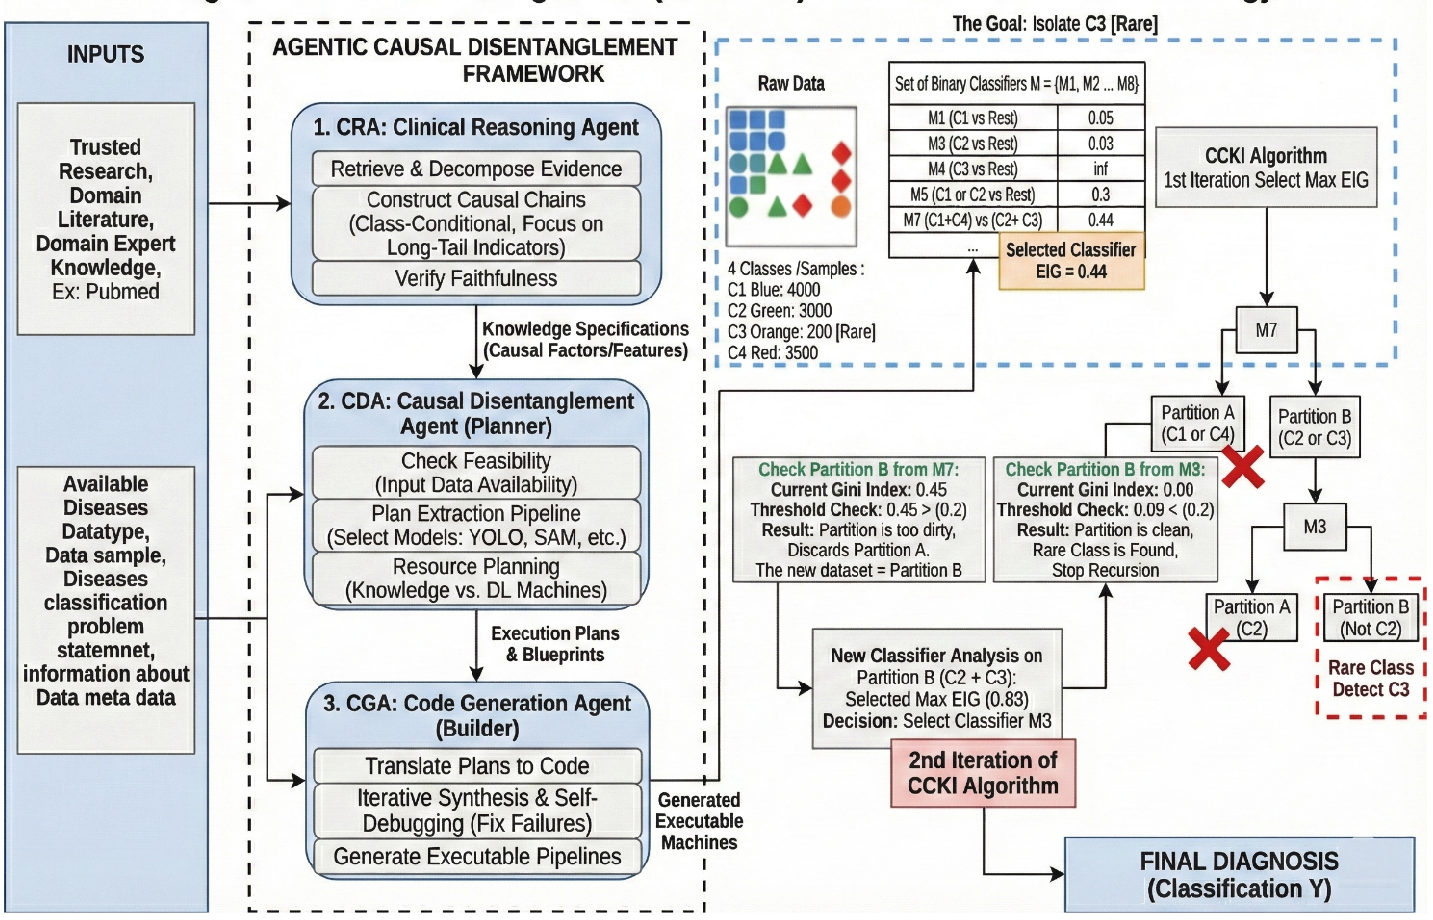
\includegraphics[width=0.75\textwidth]{flow.png}
    \vspace{-2mm}
    \caption{\scriptsize\textbf{Overview of the Agentic Causal Disentanglement (ACD) Framework with Class-Conditional Knowledge Integration (CCKI).}
The framework integrates domain knowledge and data-driven learning through three coordinated agents: (1) a Clinical Reasoning Agent that retrieves evidence and constructs class-conditional causal chains, (2) a Causal Disentanglement Agent that plans feature extraction and model selection under data and resource constraints, and (3) a Code Generation Agent that implements executable pipelines. The CCKI algorithm iteratively selects classifiers using expected information gain (EIG) to isolate rare classes via recursive partitioning, improving robust and interpretable final diagnosis under class imbalance and domain shift.}
    \label{fig:medxai_framework}
\end{figure*}
\section{Class Conditional Knowledge Integration}
We assume that we have a set of hypotheses: $H(X) = \{h_1(X), \ldots, h_m(X)\}$, some of which are data-driven hypotheses (e.g., deep learning models), while others are purely knowledge-driven (e.g., clinical knowledge in medical imaging). Without loss of generality, let $h_i(x)$ for all $i \le m_k$ be knowledge-driven, while the remaining hypotheses are data-driven. For each class $y_j \in \mathcal{Y}$, let $\phi_{y_j}$ be an if-then-else rule that combines $H(X)$ to obtain a class-specific hypothesis for $y_j$. The if-then-else combinator can be learned as a path in a decision tree that performs the following sequential steps:
\begin{itemize}
\item \textbf{Step 1:} apply a hypothesis from the set $H(X)$,
\item \textbf{Step 2:} decide if it predicts class $y_j$ or not,
\item \textbf{Step 3:} evaluate the purity of the decision,
\item \textbf{Step 4:} if purity exceeds a threshold then terminate the branch,
\item \textbf{Step 5:} else continue with a new $h(X)$ and repeat Step 1.
\item \textbf{Stopping condition:} The tree may be stopped at a specific depth $b_j$ for class $y_j$.
\end{itemize}

Let $h_{i_t}$ be the hypothesis applied at depth $t$ of the conditional branch of the decision tree.
We define an admission function for class $y_j$ at step $t$ as
\[
\alpha_{j,t}(x) \;=\; \mathbb{I}\!\left(h_{i_t}(x)=y_j\right),
\]
where $\mathbb{I}(\cdot)$ is an indicator. Let $\pi_{j,t}(x)\in[0,1]$ denote a purity/confidence score
of the hypothesis $h_{i_t}$ for class $y_j$, and let $\theta_j$ be a class-specific purity threshold.
We define the \emph{first-conclusive-step gate} as:
{\scriptsize
\begin{equation}
\label{eqn:CCKII}
\psi_{j,t}(x)
=
\mathbb{I}\!\left(\alpha_{j,t}(x)=1 \;\wedge\; \pi_{j,t}(x)\ge \theta_j\right)
\cdot
\prod_{s=1}^{t-1}
\mathbb{I}\!\left(\pi_{j,s}(x)< \theta_j\right).
\end{equation}
}

\noindent\textbf{Rationale:} The above equation states that in the previous $t-1$ steps of the branch, the purity threshold was not met, but at step $t$ we achieve conclusive confidence for class $y_j$. The final class-specific hypothesis is then given by:
{\scriptsize
\begin{equation}
\label{eqn:CCKI}
\phi_{y_j}(x) = \sum\limits_{t=1}^{b_j}{\psi_{j,t}(x)\,h_{i_t}(x)}.
\end{equation}
}
\noindent Note that by construction of \eqref{eqn:CCKII}, at most one $\psi_{j,t}(x)$ can be $1$ for a fixed $(j,x)$, so \eqref{eqn:CCKI} acts as a selector over the path hypotheses. Equation \eqref{eqn:CCKI} formally describes the CCKI classifier: if $i_t \le m_k$ at any step $t$ then $h_{i_t}$ is a knowledge-driven classifier, otherwise it is a data-driven learner/model.
% =========================
% Theorem 1 (Keep, but tighten assumptions + proof)
% Theorem 2 (Replace with a correct anti-collapse proposition)
% =========================
% =========================
% Theorem 1 (MIN-CHANGE FIX) + Eq. (7)(8) corrected
% =========================

\noindent\textbf{Theorem 1.}
CCKI enables disentanglement of domain generalization and long-tail components of the per-class generalization bound
% =========================
% Theorem 2 (MIN-CHANGE FIX)
% =========================

\noindent\textbf{Theorem 2.}
CCKI approach has a higher likelihood of achieving higher joint probability distribution
$P_T(\phi_{\mathcal{Y}}(X),Y)$ than knowledge concatenation \\
$P_T([h(X),K],Y)$ in the target domain
\emph{The proofs are provided in the Supplementary materials}
 

\begin{algorithm}[t]
\scriptsize
\caption{Class-Conditional Knowledge Integration (CCKI)}
\label{alg:ccki}
\begin{algorithmic}[1]
\Require Paired dataset $(x,y)$, rare label $y_r$, thresholds $\tau_m$, $\tau_g$, $d_{th}$, early-stop $\delta$, hypothesis set $\mathcal{H}$
\State Initialize active set $\Omega \leftarrow \{(x,y)\}$
\While{$\Omega$ refines meaningfully (e.g., $|\Omega|$ large and gain improves)}
    \For{each hypothesis $h \in \mathcal{H}$}
        \State Compute $\mathrm{EIG}(h;\Omega)$ %using Eq.~\eqref{eq:eig_def_B}
    \EndFor
    \State Let $h_{(1)},h_{(2)}$ be the top-2 hypotheses by $\mathrm{EIG}(\cdot;\Omega)$
    \If{$\mathrm{EIG}(h_{(1)};\Omega)-\mathrm{EIG}(h_{(2)};\Omega) \le \tau_m$} \Comment{tie}
        \State Let $\mathcal{T}$ be the tied set (within $\tau_m$ of the best)
        \State Choose $\hat{h}=\arg\max_{h\in\mathcal{T}} \mathrm{Dep}(h;\Omega)$ %using Eq.~\eqref{eq:dep_def}
        \If{$\mathrm{Dep}(\hat{h};\Omega) \ge d_{th}$}
            \State $h^* \leftarrow \hat{h}$
        \Else
            \State $h^* \leftarrow h_{(1)}$ \Comment{fallback}
        \EndIf
    \Else
        \State $h^* \leftarrow h_{(1)}$
    \EndIf

    \State Partition $\Omega$ by $h^*$ to obtain $S_{h^*}(\Omega)=\{\Omega^{(k)}\}_{k=1}^{K}$
    \State Select rare-enriched branch $s$ using %Eq.~\eqref{eq:rare_branch}
    \State Compute $\mathrm{Gini}(s)$
    \If{$\mathrm{Gini}(s) > \tau_g$}
        \State Update active set: $\Omega \leftarrow s$
    \Else
        \State \textbf{Stop}
    \EndIf
\EndWhile
\end{algorithmic}
\end{algorithm}
\subsection{Knowledge Extraction for Enabling CCKI}
A central challenge in realizing Class-Conditional Knowledge Integration (CCKI) lies in extracting the relevant expert knowledge required to guide model decisions. Such knowledge extraction often relies on domain experts, medical annotators, or specialized deep learning pipelines. For example, lesion- or structure-specific cues frequently require fine-tuned object-detection models such as \\
YOLO~\cite{redmon2016yolo}, SAM~\cite{kirillov2023sam}, or Detectron2~\cite{wu2019detectron2} for lesion localization, or U-Net~\cite{ronneberger2015unet} for vessel segmentation, each typically trained on expert-annotated datasets of at least 500 images per knowledge attribute. This dependence on fine-grained, pixel-level, or bounding-box annotations limits the scalability of CCKI to broader medical tasks where such resources are scarce or prohibitively expensive. Therefore, a promising next direction is to develop an agentic framework called  \textbf{\textit{Agentic Causal Disen-
tanglement (ACD)}}, capable of autonomously constructing these pipelines, retrieving domain-specific cues, and organizing them into structured priors for CCKI, thereby significantly reducing manual human involvement.
\section{Proposed Method: Agentic Causal Disentanglement (ACD)}
We propose the \textbf{Agentic Causal Disentanglement (ACD)} framework, a modular agentic pipeline that unifies expert medical knowledge with deep neural learning to address domain shift and long-tailed imbalance (rare-class fragility) in clinical imaging tasks. ACD employs a set of LLM-driven agents to autonomously retrieve, structure, and operationalize clinical knowledge, while the downstream \textbf{Class-Conditional Knowledge Integration (CCKI)} module adaptively integrates knowledge-trained classifiers $h_{\mathrm{K}}(x)$ with deep models $h_{\mathrm{D}}(x)$ that learn visual representations. The overall workflow is illustrated in Figure~\ref{fig:medxai_framework}. 
In downstream tasks, these components are instantiated via three core agents: the \textbf{Clinical Reasoning Agent (CRA)}, the \textbf{Causal Disentanglement Agent (CDA)}, and the \textbf{Code Generation Agent (CGA)}, which jointly coordinate knowledge acquisition, hypothesis construction, and decision fusion. 
%           
\subsection{Agentic Knowledge Acquisition and Rule Encoding}
%           

We now detail the first stages of ACD: acquiring symbolic knowledge, encoding it into features and rules, and preparing it for use in CCKI hypotheses $h_{\mathrm{K}}(x)$.

\textbf{Agent~1: Clinical Reasoning Agent A
(CRA) - Medical Knowledge Retrieval.}
We employ a PubMed-based Retrieval-Augmented Generation (RAG) system to extract diagnostic criteria, lesion patterns, imaging biomarkers and evidence-based decision rules for the target clinical task, the CRA-extracted knowledge for diabetic retinopathy according to each  5 stage of DR is mapped into a candidate knowledge feature set
\[
\mathcal{K} = \{k_1, k_2, \dots, k_n\},
\]
where each $k_i$ corresponds to a measurable attribute such as ``hemorrhage present'' or ``gray matter activation'' . The agent filters $\mathcal{K}$ to retain only features that can be reliably computed from the available images or input data, producing a task-specific, practically measurable knowledge feature vector.

\textbf{Agent~2: Clinical Reasoning Agent B (CRA) - Rule Refinement.}
The textual diagnostic criteria corresponding to the retained features $\mathcal{K}$ are converted into executable symbolic rules. This step adapts the knowledge to imaging and dataset constraints by defining (1) threshold ranges, (2) confidence levels, and (3) failure-case handling for conditions such as optic disc overlap, low contrast, or motion blur. The resulting rule set is denoted
\[
\mathcal{R} = \{r_1, r_2, \dots, r_m\},
\]
where each $r_i$ specifies how one or more knowledge features in $\mathcal{K}$ should be computed and interpreted from the data. $\mathcal{R}$ is finalized based on input data quality, robustness of feature extraction, and available computational resources. \newline
\textbf{Agent~3: Causal Disentanglement Agent (CDA)}
Given the target modality and disease, the LLM identifies suitable open-source deep learning models by scanning recent publications and GitHub repositories. It proposes modality-specific architectures (e.g., ViT, CNN, transformer-based backbones), retrieves available pretrained weights, and returns a recommended configuration. When a backbone is explicitly specified by the user, the agent reuses that model instead. It also based on feature vector $\mathcal{R}$ select the $h_k(x)$ classifiers. Selection criteria include code availability, reported performance, computational cost, and suitability for the target task.

\textbf{Agent~4: Code Generation Agent (CGA).}
For each refined knowledge $r_i \in \mathcal{R}$, the agent synthesizes executable Python programs using OpenCV, PyTorch APIs, and standard detection/segmentation libraries (YOLO, SAM, Detectron, U\hbox{-}Net, etc.) to operationalize the associated knowledge features. This produces a set of candidate extraction routines
\[
\mathcal{C} = \{c_1, c_2, \dots, c_p\},
\]
each responsible for computing a subset of the symbolic feature vector $\mathcal{K}$. Automated input checks, unit tests, and fallback operations are injected to ensure consistent execution. When a program fails or produces unstable outputs, a reinforcement-driven refinement loop re-prompts the LLM to update $c_i$ until the extracted features satisfy predefined correctness constraints. The validated programs provide the reliable symbolic inputs required to train the knowledge-driven hypotheses $h_{\mathrm{K}}(x)$ used by CCKI.
Our agent does not blindly trust LLM-produced rules: it iteratively proposes candidate knowledge pipelines (e.g., biomarkers/diagnostic cues) and retains only those that yield measurable gain over the DL-only baseline, discarding non-improving candidates; thus the final   CCKI cascade uses only validated knowledge branches and otherwise defaults to DL experts, it has been demonstrated in ablation study \ref{ablation_study1}.
         
\emph{Visual Feature Extraction and Self-Verification details are clearly explained in supplementary materials}
           

\section{Experiments and Results}
We evaluate the \textbf{Agentic Causal Disentanglement (ACD)} framework across four clinically critical applications spanning neuroimaging, ophthalmology, cardiology, and electrophysiology. The detailed ACD pipeline, including prompt pseudo-code and implementation details, is provided in the supplementary material to ensure reproducibility and clarity.
\vspace{-3mm}
% ============================================================
\subsection{Application 1: Diabetic Retinopathy Grading}
% ============================================================
We evaluate our framework on 5-class diabetic retinopathy (DR) grading across APTOS, EyePACS, Messidor-1, and Messidor-2. The hypothesis pool contains ten binary classifiers: five ViT-based deep models $h_{\mathrm{D}}(x)$ (one per DR grade) and five knowledge-driven classifiers $h_{\mathrm{K}}(x)$ derived from lesion and vessel morphology rules. The \textbf{CDA} module encodes clinical priors (e.g., microaneurysm burden, hemorrhage severity, vessel tortuosity), \textbf{CGA} uses YOLOv11-based detectors and vessel analysis routines to instantiate these priors as features, and CCKI organizes $h_{\mathrm{D}}(x)$ and $h_{\mathrm{K}}(x)$ into a knowledge-guided decision cascade.

\paragraph{Results.}
Table~\ref{tab:dr_all_results} summarizes three evaluation regimes: (1) \textbf{Normal DG} where we train on APTOS and test on external datasets; (2) \textbf{Single-Domain Generalization (SDG)}, where the model is trained on a single source dataset and evaluated on unseen target domains; and (3) \textbf{Multi-Domain Generalization (MDG)} using a leave-one-domain-out protocol (train on three datasets, test on the held-out one). Across all settings, our knowledge-guided fusion (ACD/CCKI) consistently improves cross-domain accuracy over the ViT-only deep branch and representative DG baselines (Fishr, SPSD-ViT), while also yielding $+5$--$6$ point gains in F1 for the rare, severe DR stages.

\begin{table}[h]
\centering
\tiny
\setlength{\tabcolsep}{4.5pt}

\caption{\textbf{Unified DR grading results across Normal DG, SDG, and MDG protocols.} 
SDG trains on a single source dataset and evaluates on unseen domains. 
MDG uses a leave-one-domain-out protocol (train on three datasets, test on the held-out one). 
Our knowledge-guided fusion consistently improves cross-domain accuracy and yields substantial gains for rare severe DR stages.}

\begin{tabular}{llllc}
\toprule
\textbf{Protocol} & \textbf{Setting} & \textbf{Method} & \textbf{Metric} & \textbf{Value (\%)} \\
\midrule
\multirow{2}{*}{Normal DG} 
  & APTOS $\rightarrow$ E+M1+M2
  & DL Branch (ViT) & Accuracy & 78.4 \\
  & APTOS $\rightarrow$ E+M1+M2
  & \textbf{Ours (ACD/CCKI)} & \textbf{Accuracy} & \textbf{84.69 $\pm$ 0.3} \\
\midrule
\multirow{12}{*}{SDG} 
  & Source: APTOS 
  & DL Branch (ViT) & Accuracy & 53.9 \\
  & Source: APTOS 
  & Ours (ACD Fusion) & Accuracy & \textbf{59.9} \\
  & Source: APTOS 
  & Best DG baseline (SD-ViT) & Accuracy & 58.6 \\[0.2em]
  & Source: MESSIDOR-1 
  & DL Branch (ViT) & Accuracy & 57.0 \\
  & Source: MESSIDOR-1 
  & Ours (ACD Fusion) & Accuracy & \textbf{67.1} \\
  & Source: MESSIDOR-1 
  & Best DG baseline (SPSD-ViT) & Accuracy & 55.9 \\[0.2em]
  & Source: MESSIDOR-2 
  & DL Branch (ViT) & Accuracy & 41.1 \\
  & Source: MESSIDOR-2 
  & Ours (ACD Fusion) & Accuracy & \textbf{65.5} \\
  & Source: MESSIDOR-2 
  & Best DG baseline (SPSD-ViT) & Accuracy & 62.1 \\[0.2em]
  & Source: EYEPACS 
  & DL Branch (ViT) & Accuracy & 50.6 \\
  & Source: EYEPACS 
  & Ours (ACD Fusion) & Accuracy & 61.7 \\
  & Source: EYEPACS 
  & Best DG baseline (SPSD-ViT) & \textbf{Accuracy} & \textbf{62.5} \\
\midrule
\multirow{5}{*}{MDG} 
  & Train E+M1+M2, test APTOS 
  & Fishr (ResNet50) & Accuracy & 47.0 \\
  & Train E+M1+M2, test APTOS 
  & SPSD-ViT (T2T-14) & Accuracy & 50.0 \\
  & Train E+M1+M2, test APTOS 
  & DL Branch (ViT, DeiT-S) & Accuracy & 50.1 \\
  & Train E+M1+M2, test APTOS 
  & KL Branch (KL-CCKI) & Accuracy & 53.1 \\
  & Train E+M1+M2, test APTOS 
  & \textbf{Ours (ACD Fusion)} & \textbf{Accuracy} & \textbf{60.7} \\
\midrule
\multirow{4}{*}{MDG (Rare)} 
  & Severe Stage 3 (APTOS) 
  & DL Branch (ViT) & F1 & 45.2 \\
  & Severe Stage 3 (APTOS) 
  & \textbf{ACD (Fusion)} & \textbf{F1} & \textbf{50.1} \\
  & Severe Stage 4 (APTOS) 
  & DL Branch (ViT) & F1 & 51.8 \\
  & Severe Stage 4 (APTOS) 
  & \textbf{ACD (Fusion)} & \textbf{F1} & \textbf{57.3} \\
\bottomrule
\end{tabular}

\label{tab:dr_all_results}
\end{table}

%============================================================
\subsection{Application 2: Seizure Onset Zone Localization}
% ============================================================
\paragraph{Setup.}
For SOZ localization from rs-fMRI, Independent Components (ICs) are first extracted via Independent Component Analysis, set up by \textbf{CRA}, who also encodes neurophysiological priors into a compact knowledge feature set (K-NumC, K-ThruV, K-SparseA, K-SparseF), while \textbf{CGA} implements the corresponding extraction pipelines and a 2D CNN branch that classifies noise vs.\ non-noise ICs.
\textbf{CDA} then constructs a CCKI decision tree over the knowledge-driven classifier $h_{\mathrm{K}}(x)$ and the deep branch $h_{\mathrm{D}}(x)$ by ranking hypotheses using Entropy Imbalance Gain (EIG).
Under extreme rare-class imbalance (approximately 5 SOZ ICs per subject), and uses Gini impurity to decide whether further refinement via the DL branch is required.
\textbf{Results.} Table~\ref{tab:soz_results} summarizes performance. The fused ACD model achieved 84.6\% accuracy and 89.7\% sensitivity, outperforming the baseline. Following the IC triage effort metric of Kamboj \etal~\cite{kamboj2024expertTAI}, our framework reduced expert review from 110 ICs to 18 ICs per subject, corresponding to an 84.2\% workload reduction.  \textbf{Cross-center generalization} was evaluated on the private datasets by training it on Phoenix Children’s Hospital (PCH) dataset and testing on an unseen University of North Carolina (UNC) dataset without fine-tuning. Performance remained stable (87.5\% accuracy), even though the DL branch degraded from 80\% to 70\% noise classification accuracy. Since the SOZ class itself is a rare class, the overall accuracy reflects an improvement as well.
\begin{table}[!htbp]
\centering
\footnotesize
\captionsetup{font=footnotesize}

\caption{SOZ localization performance. The CCKI based model's decision tree under ACD framework significantly outperforms individual components and baselines.}
\begin{tabular}{lccc}
\toprule
\textbf{Method} & \textbf{Acc (\%)} & \textbf{Sens (\%)} & \textbf{Effort} \\
\midrule
DL Branch (2D CNN Baseline)~\cite{kamboj2024expert} & 46.1 & 48.9 & 110 \\
\textbf{ACD (Ours)} & \textbf{84.6} & \textbf{89.7} & \textbf{18} \\
\bottomrule
\end{tabular}

\label{tab:soz_results}
\end{table}
\vspace{-11mm}
\subsection{Application 3: Cardiac Function Assessment}
\textbf{Setup.} For cardiac function assessment, we apply the Agentic Causal Disentanglement (ACD) Framework to the task of estimating left-ventricular ejection fraction (LVEF) from apical four-chamber echocardiogram videos. Unlike a standard deep learning model which treats the video as an end-to-end regression problem, our ACD pipeline integrates clinical knowledge describing ventricular anatomy and beat-to-beat temporal structure, inspired by the clinical workflow in the EchoNet-Dynamic paper \cite{ouyang2020echodynamic}. Specifically:
The \textbf{(CRA)} derives expert‐aligned segmentation of the left ventricle and localises cardiac cycle boundaries. The \textbf{(CDA)} disentangles anatomical structure from temporal/hemodynamic factors, thereby reducing domain‐shift and long-tail failure. The \textbf{(CGA)} gives code for extracting deep spatio-temporal features with the expert‐derived cycle-wise summaries and enforces a beat-by-beat aggregation policy rather than single‐clip regression.

We train and validate on the publicly available EchoNet-Dynamic dataset from Stanford \cite{echonetdataset}, following the same split protocol as the baseline deep network.
\textbf{Results.}  
Since the goal of ACD is generalizable knowledge integration rather than hand-tuned video optimization, its performance remains slightly below the original EchoNet-Dynamic results but maintains clinically meaningful accuracy. Our measured ACD results are shown in Table~\ref{tab:cardiac_results}.
\begin{table}[!htbp]
\centering
\footnotesize
\setlength{\tabcolsep}{3pt} % tighter spacing
\caption{LVEF estimation and heart-failure classification. ACD approaches, but does not surpass, the optimized EchoNet-Dynamic pipeline, achieving similar HF AUC while maintaining realistic EF error but with reduced model engineering cost.}
\begin{tabular}{lcc}
\toprule
\textbf{Method} & \textbf{EF MAE / Beat Var (\%)} & \textbf{HF AUC} \\
\midrule
EchoNet-Dynamic & 4.1 / 6.0 / 2.6 (6.4) & 0.97 \\
\textbf{ACD (Ours)} & 4.8 / 6.6 / 3.1 (5.9) & 0.94 \\
\bottomrule
\end{tabular}
\label{tab:cardiac_results}
\end{table}

\vspace{-11mm}
\subsection{Application 4: Coronary Artery Disease Detection from ECG}
% ============================================================

\paragraph{Setup.}
For automated diagnosis of Coronary Artery Disease (CAD), we evaluate the \textbf{(ACD)} framework using Exercise Stress ECG (ESE) data from the Mayo Integrated Stress Center (MISC) database. 
Traditional convolutional and vision transformer models (ViTs) often fail to capture domain-specific temporal and physiological nuances essential for ischemic event detection. 
To address this, ACD integrates domain knowledge from cardiologists through two causal knowledge agents: the \textbf{(CRA)} and the \textbf{(CDA)}.
In practice, expert knowledge was incorporated into the model through \textbf{lead selection masks} and \textbf{MET-level encoding}, reflecting clinicians’ understanding of ischemic signal relevance. 
This guided the transformer’s attention toward clinically meaningful ECG regions, thereby reducing noise and false positives.  
All models were trained on 726 subjects and tested on 227 unseen cases, following the same data split protocol as prior work that resulted in average 10\% greater performance than the baselines. 

\begin{table}[!htbp]
\centering
\scriptsize
\setlength{\tabcolsep}{4pt} % reduce column spacing
\caption{CAD detection results on ESE dataset. ACD integrates expert priors via lead and MET masking, yielding superior results}
\begin{tabular}{lccc}
\toprule
\textbf{Method} & \textbf{Knowledge} & \textbf{PPV / NPV / AUC (\%)} \\
\midrule
Manual Diagnosis & Human-only & 77.0 / 96.0 / – \\
DL Branch (ViT Baseline) & None & 79.0 / 81.8 / 82.0 \\
\textbf{ACD (Ours)} & \textbf{Lead + MET masks} & \textbf{91.2 / 93.0 / 92.2} \\
\bottomrule
\end{tabular}

\label{tab:cad_results}
\end{table}
\vspace{-11mm}
\section{Ablation Studies}

% ============================================================
\noindent\textbf{Ablation I (Hypothesis pool composition in CCKI).}
We evaluate how the composition of the CCKI hypothesis pool $\mathcal{H}$ affects performance on APTOS in the standard 5-class DR setting (stages 0--4). The pool includes deep hypotheses $h_{\mathrm{D}}(x)$ (ViT image classifiers) and knowledge hypotheses $h_{\mathrm{K}}(x)$ (Gradient Boosting over the fixed clinical feature vector $\mathcal{K}$ selected in Ablation I); we vary (i) the number of deep vs.\ knowledge hypotheses and (ii) prediction granularity (single 5-class predictor vs.\ five one-vs-rest binary specialists). Table~\ref{tab:aptos_ccki_ablation} shows the best configuration is \textbf{one 5-class deep hypothesis + five binary knowledge hypotheses} (A2), achieving the highest AUC ($84.65\pm0.30$), while binary-only mixtures underperform due to conflicting cascade decisions, and single-family baselines (deep-only or knowledge-only) lose complementary information.
\vspace{-4mm}
\begin{table}[!htbp]
\centering
\scriptsize
\captionsetup{font=scriptsize}
\setlength{\tabcolsep}{1pt}

\caption{\textbf{Ablation of CCKI hypothesis pool composition on APTOS (5-class DR classification).} We report AUC (mean$\pm$std). The best pool combines one 5-class deep hypothesis with five binary knowledge hypotheses (A2).}
\begin{tabular}{lccc}
\toprule
\textbf{Condition} &
\textbf{\# Deep $h_{\mathrm{D}}(x)$} &
\textbf{\# KL $h_{\mathrm{K}}(x)$} &
\textbf{AUC (\%)} \\
\midrule

\textbf{A1: 5-class $h_{\mathrm{D}}(x)$ + 5-class $h_{\mathrm{K}}(x)$} &
1 & 1 &
$83.24 \pm 0.60$ \\

\textbf{A3: binary $h_{\mathrm{D}}(x)$ + binary $h_{\mathrm{K}}(x)$} &
5 & 5 &
$81.49 \pm 0.30$ \\

\textbf{A2: binary $h_{\mathrm{K}}(x)$ + 5-class $h_{\mathrm{D}}(x)$} &
1 & 5 &
$\mathbf{84.65 \pm 0.30}$ \\

\textbf{A4: binary $h_{\mathrm{D}}(x)$ + 5-class $h_{\mathrm{K}}(x)$} &
5 & 1 &
$78.05 \pm 0.76$ \\

\textbf{A5: 5-class $h_{\mathrm{D}}(x)$ only} &
1 & 0 &
$78.74 \pm 0.98$ \\

\textbf{A6: 5-class $h_{\mathrm{K}}(x)$ only} &
0 & 1 &
$80.63 \pm 0.13$ \\

\bottomrule
\end{tabular}

\label{tab:aptos_ccki_ablation}

\end{table}`
\vspace{-2mm}

\noindent\textbf{Ablation II (Selecting symbolic knowledge for $h_{\mathrm{K}}(x)$).}
\label{ablation_study1}
We investigate which clinical features are most suitable for constructing the CCKI knowledge hypothesis $h_{\mathrm{K}}(x)$ by training five classical classifiers on the APTOS dataset using two feature families: (i) lesion biomarkers (exudates, hard/soft hemorrhages, cotton wool spots) and (ii) lesions combined with retinal vein morphology (tortuosity, caliber, branching angles). Table~\ref{tab:ablation_symbolic} shows that lesion-only features consistently outperform the combined lesions+vein features across all models. Among the evaluated methods, Gradient Boosting achieves the best performance (Acc 0.8465, F1 0.8412). Incorporating vein morphology leads to a consistent decrease in both accuracy and F1 across all classifiers, suggesting these features introduce domain-sensitive variability rather than stable class-conditional structure.

Based on this empirical evidence, we adopt \textbf{Gradient Boosting trained on lesion biomarkers only} as the canonical knowledge classifier $h_{\mathrm{K}}(x)$ used throughout the CCKI module for diabetic retinopathy analysis. This study further demonstrates that not all clinical knowledge components contribute positively to model generalization. The proposed ACD framework automatically evaluates and integrates useful knowledge components through CCKI, retaining only those that improve predictive performance.
\begin{table}[!h]
\centering
\scriptsize
\vspace{0.25em}
\setlength{\tabcolsep}{3pt}
\caption{\textbf{Ablation on symbolic lesion biomarkers with and without retinal vein features on APTOS.} Lesion-only features provide the strongest and most stable performance across models; adding vein morphology degrades accuracy and F1.}
\begin{tabular}{l|c|c|c|c|c|c}
\toprule
\textbf{Model} & \textbf{Feature Set} & \textbf{Acc} & \textbf{F1} & \textbf{Prec} & \textbf{Rec} & \textbf{AUC} \\
\midrule
Logistic Reg. & Lesions only      & 0.7732 & 0.7322 & 0.59 & 0.49 & 0.74 \\
Random Forest & Lesions only      & 0.8169 & 0.8115 & 0.82 & 0.80 & 0.81 \\
SVM           & Lesions only      & 0.7814 & 0.7432 & 0.59 & 0.50 & 0.76 \\
Grad. Boost.  & Lesions only      & \textbf{0.8465} & \textbf{0.8412} & \textbf{0.82} & \textbf{0.76} & \textbf{0.84} \\
KNN           & Lesions only      & 0.7814 & 0.7896 & 0.63 & 0.56  & 0.77 \\
\midrule
Logistic Reg. & Lesions + vein    & 0.6424 & 0.6019 & 0.25 & 0.33 & 0.58 \\
Random Forest & Lesions + vein    & 0.7384 & 0.7038 & 0.55 & 0.47 & 0.70 \\
SVM           & Lesions + vein    & 0.6556 & 0.6083 & 0.26 & 0.34  & 0.58 \\
Grad. Boost.  & Lesions + vein    & 0.7252 & 0.7389 & 0.51 & 0.44 & 0.69 \\
KNN           & Lesions + vein    & 0.6987 & 0.6369 & 0.43 & 0.44 & 0.66 \\
\bottomrule
\end{tabular}

\label{tab:ablation_symbolic}
\end{table}
%\vspace{-1mm}

\noindent\textbf{Ablation III (Comparison with ensemble and mixture-of-experts baselines).}
\label{app:kittler_moe}
To further verify that the performance gains of CCKI are not explained by standard model combination strategies, we compare against two commonly used multi-model paradigms: \textbf{ensemble learning} and \textbf{mixture-of-experts (MoE)}. The ensemble baseline averages predictions from multiple independently trained classifiers, while the MoE baseline uses a learned gating network to combine expert predictions. All methods are trained under the same protocol using the identical ViT backbone and training configuration. As shown in Table~\ref{tab:ensemble_ablation}, traditional ensemble learning achieves 77.90\% accuracy and the MoE approach improves performance to 81.90\%. However, our proposed \textbf{CCKI} framework achieves the highest accuracy of \textbf{84.78\%}. This improvement indicates that structured neuro-symbolic reasoning within the CCKI cascade enables more effective integration of complementary hypotheses than generic ensemble aggregation or gating-based expert mixtures.

\begin{table}[!htbp]
\centering
\scriptsize
\setlength{\tabcolsep}{6pt}
\caption{\textbf{Comparison with ensemble-based model combination strategies.} Our structured CCKI framework outperforms both standard ensemble learning and mixture-of-experts baselines.}
\begin{tabular}{lc}
\toprule
\textbf{Method} & \textbf{Accuracy (\%)} \\
\midrule
Ensemble Learning & 77.90 \\
Mixture of Experts (MoE) & 81.90 \\
\textbf{CCKI (Ours)} & \textbf{84.78} \\
\bottomrule
\end{tabular}

\label{tab:ensemble_ablation}
\end{table}

\vspace{-10mm}
\section{Conclusion and Discussion}
\label{sec:conclusion}

This paper studies a clinically realistic setting where \emph{domain shift} and \emph{long-tailed imbalance} co-occur, and where improving one objective can degrade the other. We formalize this tension through a per-class DG risk characterization showing that rare classes suffer disproportionately because both limited class support and class-conditional domain divergence inflate target risk. We further interpret the conflict as an optimization mismatch: domain generalization tends to favor flatter, domain-invariant solutions, while long-tail learning amplifies minority gradients, inducing sharper minima and gradient misalignment.

To address this, we propose \textbf{Class-Conditional Knowledge Integration (CCKI)}, a decision cascade that routes predictions through deep and knowledge-driven hypotheses using a first-conclusive-step gating mechanism, rather than naive feature concatenation. Building on CCKI, we introduce \textbf{Agentic Causal Disentanglement (ACD)}, a coordinated multi-agent framework that (i) retrieves clinically grounded priors, (ii) operationalizes them into computable biomarkers and causal factors, and (iii) validates the resulting pipelines before integration with deep predictors.  
%%%%%%%%%%%%%%%%%%%%%%%%%%%%%%%%%%%%%%%%%%%%%%%%%%%%%%%%%%%%%%%%%%%%%%%%%%%%%%%%%%%%%%%%%%%%%%%%

\bibliographystyle{splncs04}
\bibliography{main}
% WARNING: do not forget to delete the supplementary pages from your submission 
% \input{sec/X_suppl}


\end{document}
